\section{Auswertung}
\label{sec:Auswertung}

Die im Versuch aufgenommenen Daten dienen nun zur Bestimmung der Aktivierungsenergie $W$ und der charakteristischen Relaxationszeit $\tau_0$.
Die Auswertung der Messungen für beide Heizraten verlaufen vollkommen gleich und werden im Folgenden parallel durchgeführt.
In \autoref{fig:plot1} ist zunächst der gemessene Relaxationsstrom in Abhängigkeit von der Temperatur aufgetragen.

\begin{figure}[H]
  \begin{subfigure}{\textwidth}
  \centering
  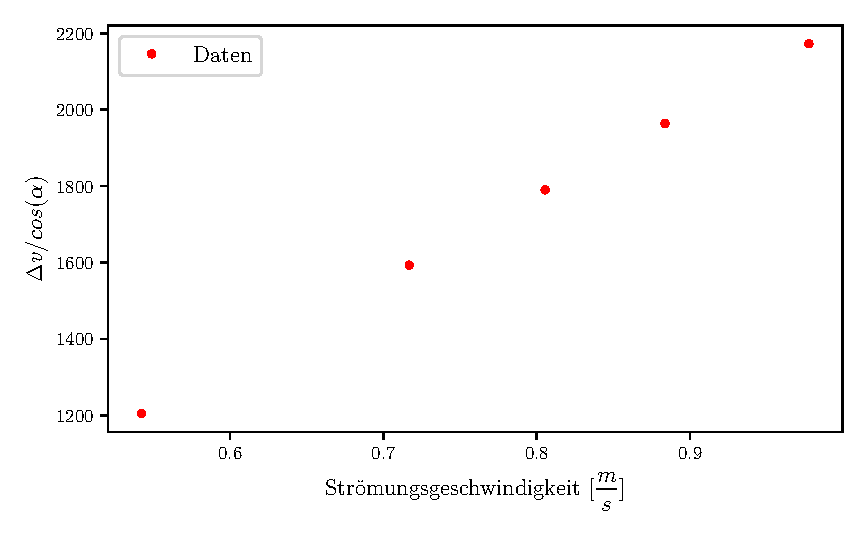
\includegraphics[width=\textwidth]{build/plot1.pdf}
  \caption{Messung 1.}
  \label{fig:plot1a}
  \end{subfigure}
  \hfill
  \begin{subfigure}{\textwidth}
  \centering
  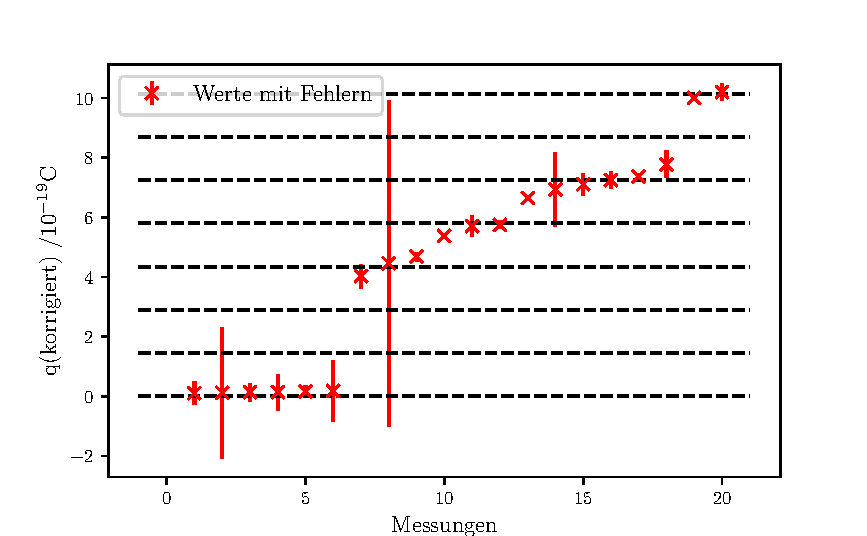
\includegraphics[width=\textwidth]{build/plot3.pdf}
  \caption{Messung 2.}
  \label{fig:plot1b}
  \end{subfigure}
  \caption{Depolarisationsstrom in Abhängigkeit von der Temperatur mit Regression für den Untergrund.}
  \label{fig:plot1}
\end{figure}

Die mittlere Heizrate berechnet sich zu
\begin{align*}
  b_1&= \qty{1.964 \pm 0.044}{\kelvin\per\minute}\\
\intertext{in Messung 1, und}
  b_2 &= \qty{1.465 \pm 0.028}{\kelvin\per\minute}\\
\intertext{in Messung 2.}
\end{align*}

Da wenige Werte im gleichen Temperaturbereich in beiden Kurven stark vom restlichen Kurvenverlauf abweichen, wird eine Regression mittels
einer Gauß-Kurve durchgeführt und die Werte entsprechend korrigiert. Im Weiteren wird nun mit den korrigierten Werten gearbeitet.
Da das erste Maximum des Relaxationsstroms, welches im Folgenden genauer
untersucht wird, auf der steigenden Flanke des zweiten Maximums liegt, wird dieser
”Untergrund” von den Messwerten abgezogen.
Das zweite Maximum entsteht durch den Dipolstrom der Wassermoleküle, welche sich bei höheren Temperaturen am Ionenkristall anlagern.
Um den Untergrund zu bestimmen wird eine Regression der Form
\begin{align*}
  f(T)= a * \text{exp}(-b/T)
\end{align*}
an den Messwerten durchgeführt die außerhalb der Maximumskurve liegen.
Der so errechnete Untergrund wird von den Messwerten abgezogen.
In \autoref{fig:plot2} sind die bereinigten Messwerte dargestellt.

\begin{figure}[H]
  \begin{subfigure}{\textwidth}
  \centering
  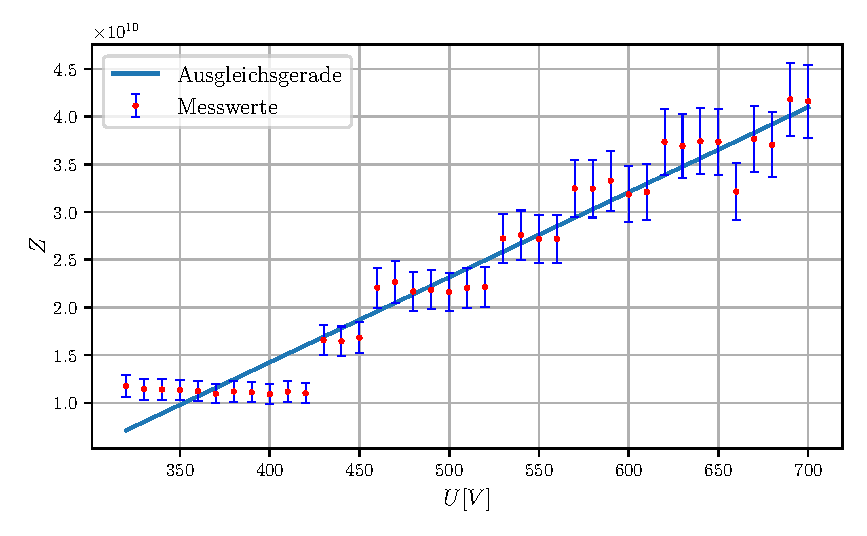
\includegraphics[width=\textwidth]{build/plot2.pdf}
  \caption{Messung 1.}
  \label{fig:plot2a}
  \end{subfigure}
  \hfill
  \begin{subfigure}{\textwidth}
  \centering
  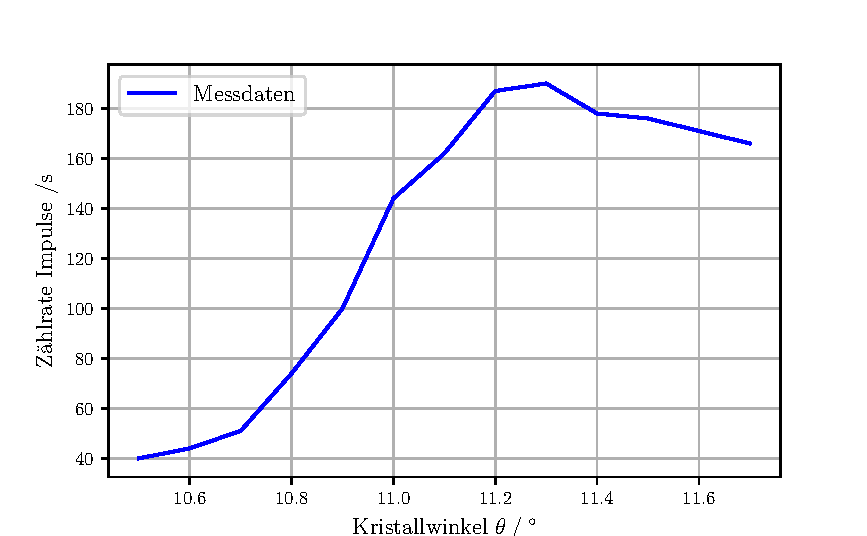
\includegraphics[width=\textwidth]{build/plot4.pdf}
  \caption{Messung 2.}
  \label{fig:plot2b}
  \end{subfigure}
  \caption{Um den Untergrund bereinigte Messwerte des Depolarisationsstroms.}
  \label{fig:plot2}
\end{figure}



\subsection{Berechnung der Aktivierungsenergie W}
\label{subsec:Aktivierungsenergie}

Die Werte die für die Bestimmung der Aktivierungsenergie $W$ mit Hilfe der Anlaufkurve des Maximums verwendet werden sind in \autoref{fig:plot2}
schwarz markiert.
Für die Bestimmung der Aktivierungsenergie unter Verwendung des gesamten Kurvenverlaufs werden sowohl die schwarz, als auch die blau
markierten Werte aus \autoref{fig:plot2} verwendet.

\subsubsection{Bestimmung mit Hilfe der Anlaufkurve des Maximums}

